
\chapter{TALEND Open Studio for Data Integration 5.6}

\section{Création du modèle OLAP}
\subsection{Question à répondre}
Analyse des ventes de bande dessinées d'une enseigne de librairie possédant plusieurs boutiques dans plusieurs villes.

\subsection{Modèle ROLAP}

L'implémentation ROLAP a été choisie par rapport au modèle MOLAP car même si la quantité de données était petite, il m'a semblé important d'étudier ce modèle qui paraît être très utilisé. Ne voyant rien justifier un modèle en flocon permettant de gagner de l'espace de stockage, j'ai utilisé un modèle en étoile.
La table de faits est la table vente. Les dimentsions sont le temps, la boutique(lieu d'achat), le client, et le livre. L'étoile est de type transaction.

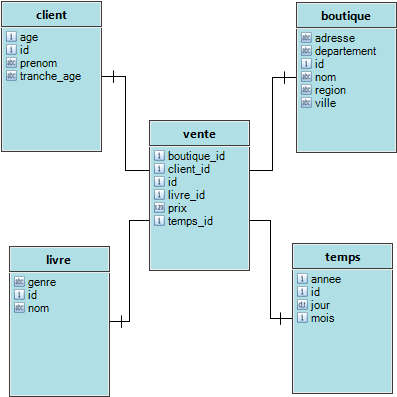
\includegraphics[clip=true, width=120mm, height=80mm]{images/Talend.png} 



\subsubsection{Table de faits vente}

\paragraph{Indicateurs}

prix de la vente; ce que le vente a rapporté

\subparagraph{fonctions d'agrégat}
\begin{itemize}
\item addition sur le prix
\item moyenne sur le prix
\end{itemize}


\paragraph{Dimension client}

\begin{itemize}
\item id
\item prenom
\item age
\item tranche\_age ("-12", "12-25", "35-65", "25-34", "+65")
\end{itemize}

\subparagraph{hiérarchie}
 age $<$ tranche\_age

\paragraph{Dimension boutique}
\begin{itemize}
\item id
\item nom
\item adresse
\item departement
\item ville
\item region
\end{itemize}

\subparagraph{hiérarchie}
adresse $<$ ville $<$ department $<$ region

\paragraph{Dimension livre}
\begin{itemize}
\item id
\item nom
\item genre
\end{itemize}

\subparagraph{hiérarchie}
nom $<$ genre

\paragraph{Dimension Temps}

\begin{itemize}
\item id
\item jour
\item mois
\item annee
\end{itemize}

\subparagraph{hiérarchie}
jour $<$ mois $<$ annee

\section{Intégration avec TALEND}

\subsection{Téléchargement Installation}
Le téléchargement se fait sur \url{http://fr.talend.com/download/data-integration}.
La documentation de l'outil est disponible au même endroit dans la partie Manuels d'utilisateurs et est facilement accessible.
L'outil est en fait basé sur Eclipse ce qui le rend facilement appréhendable pour ceux qui connaissent le célèbre IDE mais vient aussi avec ses défauts.

\subsection{Méthode utilisée}

Pour chaque dimension, j'ai essayé d'avoir un cas d'usage différent:
\begin{itemize}
\item La dimension livre se construit par une jointure classique entre deux tables. 
\item La dimension client est construite en utilisant la table client suivie d'une transformation sur l'un de ses champs afin de déduire la tranche d'age à partir de l'age.
\item La dimension boutique utilise des sources de données de type différents (CSV et postgres).
\item La dimension temps construite à partir de la table temps subit un action sur ses données afin d'enlever les doublons et de déterminer les hiérarchies à partir d'une date.
\end{itemize}

\subsection{Configuration des sources de données}
Talend doit se connecter à la base de données postgres en lecture d'une part pour lire les données des tables de la base de données OLTP, d'autre part pour écrire en base dans la base de données de type ROLAP.\\
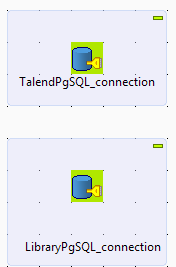
\includegraphics[scale=1]{images/db_connection.PNG}\\
La source CSV est toute aussi facile à configurer. Il suffit de configurer le séparateur, la présence ou non d'une entête et les colonnes à prendre en compte comme le montre la figure ci-dessous:\\

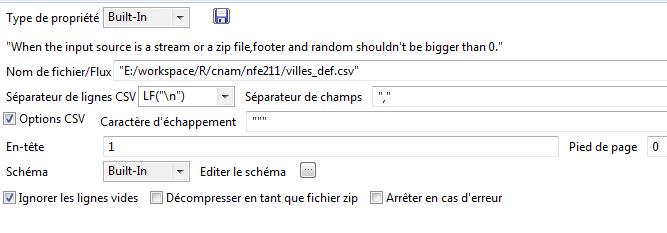
\includegraphics[scale=0.60]{images/csv.PNG}

\subsection{Dimension Boutique}
\subsubsection{Difficulté testée}
La difficulté ici est de lier des données entre deux sources de données de type différents : CSV et Database.

\subsubsection{Mise en œuvre}
Les deux sources de données configurées nous permettent de faire une jointure simple avec le composant tMap. Le lien entre les entités se fait de manière intuitive sur cet écran:

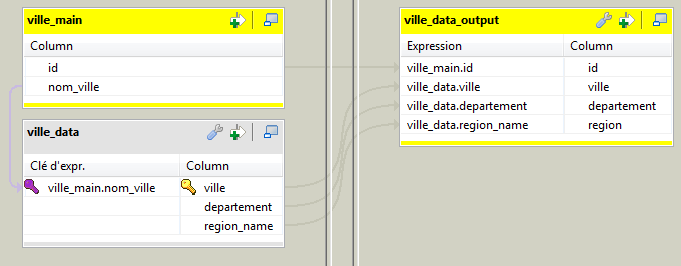
\includegraphics[scale=0.60]{images/ville_mappingcsv.PNG}\\
Dans la suite de ce projet nous utiliserons toujours une tMap pour faire une jointure entre deux sources de données.\\
Nous pouvons conclure que TALEND ne fait pas de distinction entre les différents types de données pourvu qu'elle soit composée de colonnes.

\subsection{Dimension Livre}
\subsubsection{Difficulté testée}
Aucune, jointure simple entre deux tables d'une base de données.

\subsubsection{Mise en œuvre}
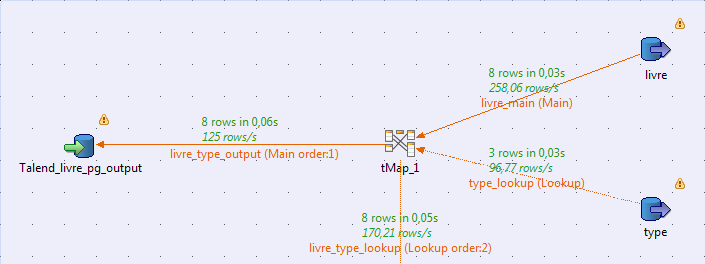
\includegraphics[scale=0.60]{images/dimension_livre.PNG}

\subsection{Dimension Client}
\subsubsection{Difficulté testée}
La dimension client est construite en utilisant la table client suivie d'une transformation sur l'un de ses champs afin de déduire la tranche d'age à partir de l'age.

\subsubsection{Mise en œuvre}
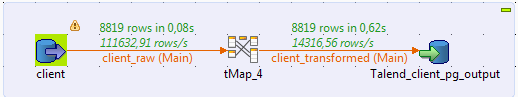
\includegraphics[scale=0.60]{images/dimension_client.PNG}\\

Pour transformer un age en tranche d'age, nous avons besoin de créer une routine dont le code est montré en annexe \ref{toTrancheDage} .

\subsection{Dimension Temps}
\subsubsection{Difficulté testée}
La dimension temps construite à partir de la table temps subit un action sur ses données afin d'enlever les doublons et de déterminer les hiérarchies à partir d'une date.
\subsubsection{Mise en œuvre}
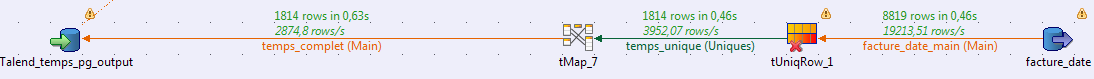
\includegraphics[scale=0.60]{images/dimension_temps.PNG}\\
Le composant tUniqRow\_ que nous voyons sur ce schéma sert à enlever les doublons. C'est à dire que nous voulons une seule date dans notre dimension temps. Nous prenons donc l'ensemble des dates distinctes trouvées dans la table facture.
Une fois ces dates trouvées, nous voulons déterminer les hiérarchies à partir du champs date\_achat de la table facture. Nous utilisons pour cela les fonctions built-in de TALEND :
\begin{itemize}
\item TalendDate.getPartOfDate("MONTH", date\_achat) pour déterminer le mois d'une date
\item TalendDate.getPartOfDate("YEAR", date\_achat)
\end{itemize}

\subsection{Table de faits vente}
\subsubsection{Difficulté testée}
Aucune, l'intégrité relationnelle des données est gérée côté base OLTP, ce qui réduit la création de la table de faits à un ensemble de jointure.
\subsubsection{Mise en œuvre}
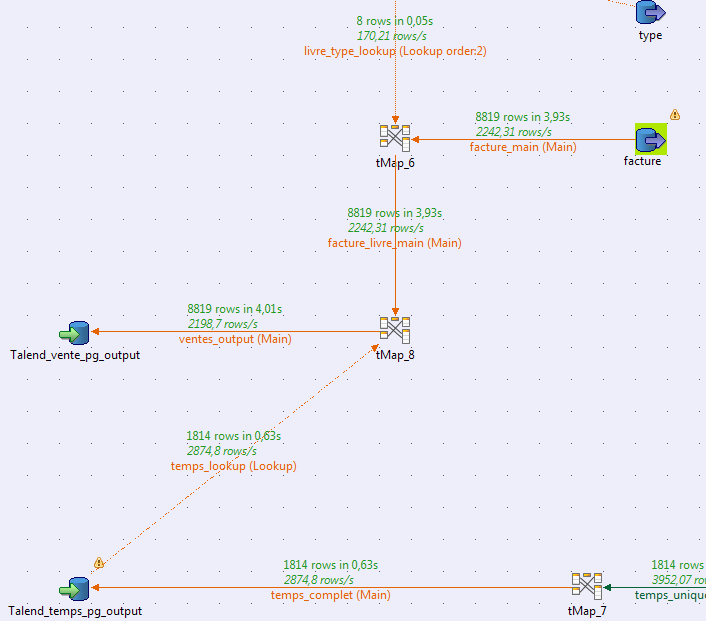
\includegraphics[scale=0.70]{images/table_faits_vente.PNG}

Aucune jointure avec la table client et la table boutique n'est nécessaire puisque les relations sont prises directement de la base OLTP et qu'aucune transormation sur les clés étrangères n'est effectuée.

\subsection{Conclusion sur l'utilisation de TALEND}
Pour les cas testés qui paraissent classiques, TALEND se montre plutôt efficace. La montée en charge reste à tester. Le nombre de composant paraît énorme et je n'ai pas réussi à les utiliser tous. C'est d'ailleurs un des défauts de TALEND à mon sens. L'utilisation n'est pas très intuitive et la résolution de problème est très compliquée. Lorsqu'un problème survient, l'utilisateur est gratifié d'un NullPointerException sans plus d'information. La modification du code JAVA généré est anecdotique selon moi même si son utilité est révélée lorqu'il s'agit de débugger. 
 
\clearpage